\chapter{Asking a 27-Year-Old How to Make \$300 Million}

These notes follow a School of Hard Knocks interview with Zane, curated by LazyingArt LLC with Video2Book. There is no validated board work or mathematical screenshot for this lecture, so the formal structure below comes from the transcript itself: stated numbers, thresholds, ratios, and mechanisms. We read the interview as a source-conscious case study in scale: what was claimed, what operating rule was offered, and how the arithmetic sharpens the business judgment without turning the interview into a textbook theory.

\section{The Opening Number}

The interview begins with the result before the origin story. The host asks whether Zane is the chief executive of one of the largest solar companies in the country, then asks for the largest amount of money the business has made in a single year. Zane says the business did \(\$149\mathrm{M}\) last year and should roughly double that this year.

The arithmetic is simple, but it is the first anchor:
\begin{equation}
149\,\mathrm{M}\times 2 = 298\,\mathrm{M}\approx 300\,\mathrm{M}.
\end{equation}
This is interview testimony, not independently verified financial reporting. Its purpose in the lecture arc is to set the scale of the object we are studying. Before we ask what wealth is, or how it should be used, we ask what kind of organization could plausibly move from one large annual revenue number to the next.

The operating context appears almost immediately after the introduction. Zane describes a residential solar installation company in Miami with more than \(600\) W2 employees and more than \(3000\) sales representatives selling through it:
\begin{equation}
\text{W2 employees}>600,\qquad \text{sales reps}>3000.
\end{equation}
That distinction matters. The company is not presented as a solo operator with a large audience. It is presented as an organization: employees, distributed sales capacity, and repeatable field execution.

\section{From Salesperson to Owner}

The host then pulls the story backward. Zane says he grew up lower class, with first-generation immigrant parents who did not speak English. At eighteen he decided to go all in on sales, then entered solar sales. The path he gives is compact:
\begin{equation}
\text{salesperson}\longrightarrow \text{sales leader}\longrightarrow \text{business owner}.
\end{equation}

The first money-making mechanism is therefore not inheritance, financial engineering, or a protected technical invention. It is sales. In these notes, sales is the first conversion function: it turns a conversation with a customer into revenue, and it turns personal effort into commercial leverage. Zane's account places that skill before systems, networks, reinvestment, and even the later definition of wealth.

This is the first recurrence in the interview. A person can make money by selling. A company becomes valuable only when the selling is embedded in a structure that can survive beyond one person's day-to-day effort. The next question asks how that structure appears.

\section{Seven, Eight, and Nine Figures}

The first major operating question is about scale. The host asks what allowed the business to move from seven figures to eight figures and then toward nine figures. Zane answers with a ladder. We can preserve the rhythm of the answer as a sequence of operating regimes:
\begin{align}
7\text{-figure scale} &\Rightarrow \text{idea}+\text{sales}+\text{marketing},\\
8\text{-figure scale} &\Rightarrow \text{team},\\
9\text{-figure scale} &\Rightarrow \text{product}+\text{marketing}+\text{sales}+\text{team}+\text{systems/SOPs}.
\end{align}

The implication sign here is qualitative. It does not mean that every seven-figure business has the same anatomy, or that every nine-figure business obeys the same rule. It records Zane's operating claim: as scale rises, the limiting factor changes. At first the founder can carry much of the load. Then the team must carry it. Finally the system must carry it.

\begin{figure}
\centering
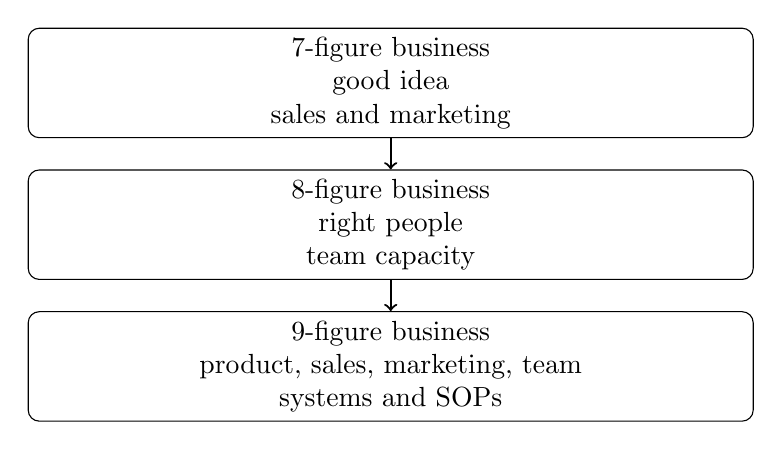
\begin{tikzpicture}[
  node/.style={draw, rounded corners, align=center, text width=.74\linewidth, minimum height=1.0cm},
  arrow/.style={->, thick}
]
\node[node] (a) at (0,0) {\(7\)-figure business\\good idea\\sales and marketing};
\node[node] (b) at (0,-1.8) {\(8\)-figure business\\right people\\team capacity};
\node[node] (c) at (0,-3.6) {\(9\)-figure business\\product, sales, marketing, team\\systems and SOPs};
\draw[arrow] (a) -- (b);
\draw[arrow] (b) -- (c);
\end{tikzpicture}
\caption{The scaling ladder stated in the interview, redrawn as a compact operating model.}
\end{figure}

\subsection{Question \& Answer}

\paragraph{Question.}
Why does the chief executive become the bottleneck as the business grows?

\paragraph{Answer.}
Because undocumented work stays trapped inside a person. Zane's example is deliberately exaggerated: he says there is a standard operating procedure for everything, even ordinary activities such as making coffee. The joke points to a serious mechanism. If a function is documented, another person can perform it when the original operator is absent.

\begin{definition}
A standard operating procedure, or SOP, is a written description of a business function that makes the function repeatable and transferable.
\end{definition}

The update rule is:
\begin{equation}
\text{undocumented function}
\longrightarrow
\text{documented function}
\longrightarrow
\text{transferable function}
\longrightarrow
\text{lower founder dependence}.
\end{equation}

At eight figures, Zane says, many companies still rely on the CEO. At nine figures, the reliance shifts toward the machine and the system. The strongest version of the claim is that the company should keep operating even if the CEO disappears.

\begin{figure}
\centering
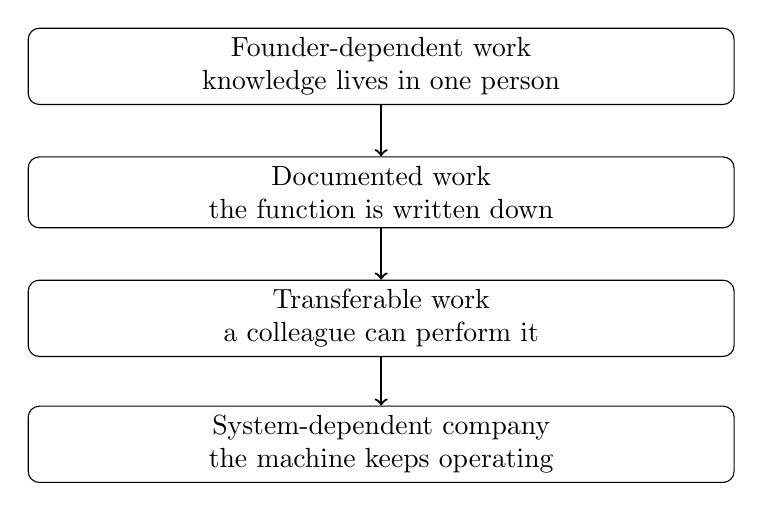
\begin{tikzpicture}[
  node/.style={draw, rounded corners, align=center, text width=.72\linewidth, minimum height=.9cm},
  arrow/.style={->, thick}
]
\node[node] (a) at (0,0) {Founder-dependent work\\knowledge lives in one person};
\node[node] (b) at (0,-1.6) {Documented work\\the function is written down};
\node[node] (c) at (0,-3.2) {Transferable work\\a colleague can perform it};
\node[node] (d) at (0,-4.8) {System-dependent company\\the machine keeps operating};
\draw[arrow] (a) -- (b);
\draw[arrow] (b) -- (c);
\draw[arrow] (c) -- (d);
\end{tikzpicture}
\caption{The founder-dependence reduction implied by Zane's SOP argument.}
\end{figure}

\section{Moving Closer to the Money}

Once the operating ladder is in place, the interview pivots from company scale to personal escape velocity. The host asks about escaping the cycle of poverty. Zane's answer is blunt: in his view, a person cannot get rich while remaining in a poor environment. We should keep that phrasing attached to him. It is a strong anecdotal claim, not a universal law.

The mechanism he gives is more useful than the slogan. First, build skill while trapped. Second, save enough money to move. Third, relocate toward a denser economy where money, customers, operators, and ambition are more visible.

The transcript gives a contrast. In one environment, everyone around you may be making about \(\$40{,}000\) per year. In another, Zane imagines a city where, within a \(30\)-mile radius, there may be \(14\) billionaires and tens of thousands of multimillionaires:
\begin{equation}
r=30\ \mathrm{miles},\qquad
N_{\mathrm{billionaires}}\approx 14,\qquad
N_{\mathrm{multimillionaires}}=\text{tens of thousands}.
\end{equation}
Those numbers should be treated as his opportunity-density example, not as verified local demographics.

The proposed mechanism is qualitative:
\begin{equation}
\text{skill}+\text{relocation}+\text{opportunity density}
\Rightarrow
\text{more chances for contact, commerce, and motivation}.
\end{equation}
Location does not guarantee success. It changes what one sees, who one meets, and what kinds of opportunities are normal enough to be pursued.

\section{Networks Require Value Before Access}

After the sponsor interruption, the interview returns to relationships. The host asks how Zane has leveraged relationships and what advice he would give someone trying to build a network. Zane answers with a hard premise: successful people focus on what adds value to their lives. If one brings no value, one should not expect value in return.

This is the second bottleneck in the lecture. Earlier, the bottleneck was founder dependence. Here the bottleneck is social value. Being in the room does not yet mean that one belongs in the room, and accidental proximity does not yet create durable access.

\subsection{Question \& Answer}

\paragraph{Question.}
Why does meeting a billionaire not automatically create a useful relationship?

\paragraph{Answer.}
Because contact is not the same thing as earned access. Zane gives the example of running into Elon Musk in the street. The meeting might be exciting. It might create content. But it does not imply a phone number, a returned call, or an ongoing channel of trust.

In compact form:
\begin{equation}
\text{accidental contact}\neq \text{durable relationship}.
\end{equation}
A more useful relationship model is:
\begin{equation}
\text{durable relationship}
\Rightarrow
\text{access}+\text{value}+\text{trust}+\text{reciprocity}.
\end{equation}

Zane then gives the negative form of the same rule. It is not only about whom one spends time with; it is also about whom one avoids. A person can be excluded from better rooms because the group around him signals negativity, unseriousness, or low value. In the transcript's language, the table one wants is a table where the conversation is about helping each other, making more money, and building real ideas.

\section{Spend Money, But Put It to Work}

The host next asks for the best financial advice Zane ever received. Zane answers with a reversal: spend your money. That sounds, at first, as if it contradicts the earlier instruction to save enough money to move. The contradiction disappears when we separate stages of capital.

At the escape stage, money is saved for skill and relocation. At the operating stage, excess cash should not sit idle after expenses, operating costs, and payroll are covered. Zane frames idle business cash as a vehicle with no fuel: impressive to look at, but not doing work.

Let \(C\) denote business cash and \(O\) denote operating requirements: expenses, payroll, and near-term obligations. The cash available for deliberate deployment is:
\begin{equation}
C_{\mathrm{excess}}=C-O.
\end{equation}
The practical rule is:
\begin{equation}
C_{\mathrm{excess}}>0
\quad\Longrightarrow\quad
\text{ask whether the money is protection or unused fuel}.
\end{equation}
If the answer is unused fuel, Zane's doctrine is to put it back into the business, into capability, or into assets:
\begin{equation}
C_{\mathrm{excess}}
\longrightarrow
\text{people}+\text{systems}+\text{capacity}+\text{skill}+\text{assets}.
\end{equation}

\subsection{Question \& Answer}

\paragraph{Question.}
How can the same interview say both ``save your money'' and ``spend your money''?

\paragraph{Answer.}
Because the words refer to different stages. In the poverty-cycle answer, saving means accumulating enough escape capital to buy skill and move closer to opportunity. In the financial-advice answer, spending means deploying excess business capital rather than admiring idle cash.

\begin{table}
\centering
\begin{tabular}{p{.34\linewidth}p{.52\linewidth}}
\hline
Use of money & Role in the interview\\
\hline
Escape savings & Build skills and move toward a denser economy\\
Consumption & Cars, watches, clothes, and status purchases are delayed\\
Idle cash & Creates comfort but may reduce urgency and discipline\\
Reinvestment & Builds the business asset and forces continued performance\\
Deployed assets & Marks Zane's stricter idea of wealth\\
\hline
\end{tabular}
\caption{The interview separates saving, consuming, holding idle cash, and deploying capital.}
\end{table}

\paragraph{Worked decision rule.}
The transcript's logic can be written as a simple operating procedure:
\begin{enumerate}
\item Cover required operating costs and payroll.
\item Compute \(C_{\mathrm{excess}}=C-O\).
\item If \(C_{\mathrm{excess}}\leq 0\), preserve liquidity and stabilize the business.
\item If \(C_{\mathrm{excess}}>0\), ask whether the cash protects a real risk or merely creates comfort.
\item If it merely creates comfort, deploy it into the business, into personal capability, or into productive assets.
\end{enumerate}

This is not general financial planning advice. It is Zane's operating doctrine for a growth business whose owner believes that the main net-worth engine is the company itself.

\section{Conviction, Riches, and Wealth}

The interview then returns to the first skill: sales. The host asks how Zane has sold at high volume across his career. Zane rejects a technique-first answer. Scripts, objection handling, and role plays matter; he says his own salespeople use them. But in his hierarchy, the controlling variable is conviction in the product.

His rough weighting is:
\begin{equation}
\text{sales effectiveness}
\approx
10\%\,(\text{tactics})+90\%\,(\text{conviction}).
\end{equation}
This is rhetoric, not measurement. Its point is that buyers sense enthusiasm, belief, and hesitation. A trained salesperson who does not believe in the product may lose to a less trained salesperson whose belief is obvious.

The interview then widens from selling to the difference between being rich and being wealthy. Zane defines ``rich'' as making roughly \(\$4\mathrm{M}\) to \(\$10\mathrm{M}\) per year. He reserves ``wealthy'' for billionaire-level assets that are deployed and working:
\begin{align}
\text{rich} &\sim \$4\mathrm{M}\text{--}\$10\mathrm{M}\ \text{per year},\\
\text{wealthy} &\sim \$1\mathrm{B}\ \text{in deployed assets}.
\end{align}

The distinction is not only numerical. It is structural. Wealth, in this answer, means money placed into businesses, private equity, stocks, real estate, and other assets. It is capital with a job.

\begin{table}
\centering
\begin{tabular}{p{.30\linewidth}p{.56\linewidth}}
\hline
Category & Zane's framing in the interview\\
\hline
Rich & High annual income, roughly \(\$4\mathrm{M}\) to \(\$10\mathrm{M}\) per year\\
Wealthy & Billionaire-level assets deployed across productive holdings\\
Risk point & Large lifestyle assets can stress smaller balance sheets\\
\hline
\end{tabular}
\caption{The rich/wealthy distinction is Zane's stated taxonomy, not a universal financial definition.}
\end{table}

His yacht example gives the cleanest ratio calculation. If a person has \(\$100\mathrm{M}\) and carries a luxury asset costing more than \(\$12\mathrm{M}\) per year to operate, then the annual operating cost is about \(12\%\) of net worth:
\begin{equation}
\frac{\$12\mathrm{M}}{\$100\mathrm{M}}
=
0.12
=
12\%.
\end{equation}
At \(\$1\mathrm{B}\), a \(\$50\mathrm{M}\) purchase is still large, but it is a smaller fraction of the balance sheet:
\begin{equation}
\frac{\$50\mathrm{M}}{\$1\mathrm{B}}
=
0.05
=
5\%.
\end{equation}
The point is not the yacht. The point is that scale changes the meaning of the same purchase. A toy that is survivable at one level can be financially distorting at another.

\section{Summary}

The interview begins with \(\$149\mathrm{M}\) and a projected path toward \(\$300\mathrm{M}\), but the number is only the opening move. Zane's explanation unfolds as a sequence: sales creates the first opportunity; team extends the business beyond the founder; SOPs turn work into transferable machinery; environment changes the density of opportunity; relationships require value before access; and money, once the base is protected, should be deployed rather than admired.

The final advice compresses the whole interview into two imperatives: learn sales and do not quit. In the chapter's terms, sales is the first skill, persistence is the long constraint, and the intervening mechanisms are what keep personal effort from remaining merely personal. The \(\$149\mathrm{M}\), \(\$300\mathrm{M}\), \(600\)-employee, \(3000\)-rep, \(10/90\), and yacht-cost examples should remain attached to the transcript as claims and illustrations. Their value is not that they prove a universal law of wealth. Their value is that they reveal one operator's commercial model for moving from personal selling to institutional scale.